% Chapter 2
\usepackage{caption}
\usepackage{subcaption}

\chapter{Problem formulation} % Write in your own chapter title
\label{Chapter2}
\lhead{Chapter 2. \emph{Problem formulation}} % Write in your own chapter title to set the page header

Climate change, pest, and diseases and all the environmental phenomena that currently affect the world, have generated different challenges to deal in the incoming years. One of those challenges is the direct impact on food security \cite{wheeler2013climate} at a global level; this has called attention at a global scale to generate  resistant crops to all these factors and at same time increasing yield and its nutritional value (plant breeders tasks) but also giving tools to farmers to increase and warrant their food production.

One selected important crop to face the food security problem is Banana \textit{(Musa spp)}\cite{faostat2014food};
Though a major staple in Africa, Asia, and Latin America, only 13\% of bananas produced are globally traded \cite{lescot2013world}, clearly indicating the fruit’s importance in domestic markets and for food security. In East and Central Africa, it is a substantial dietary component, accounting for over 50\% of daily total food intake in parts of Uganda and Rwanda\cite{abele2007bacterial}. In Colombia, Banana is one of the main fruit crops that sustain the country's food security and it as a part of different typical dishes.

A big concern in Banana are pest and diseases, and this has a direct impact on yield and food production. Several diseases affect banana crops around the world threaten food security, such as Banana bunchy top virus(BBTV), banana Xanthomonas wilt(BXW)(see figure \ref{fig:subim1}), Black and Yellow Sigatoka and Fusarium wilt and some pest as Banana Weevil(see figure \ref{fig:subim2}). In order to manage the spread of crop diseases and pest, early identification in the field is a crucial step. Fortunately, most of the crop diseases can be managed by detecting the diseases as soon as it appears on the crop. Traditional pest and disease identification approaches rely on the support of agricultural extension specialists, but these approaches are limited in developing countries with low human infrastructure capacity. The major part of banana crops around the world are from smallholders farmers; they do not know, or they use empirical methods to make the diagnosis, but the early identification of the problem is not possible in most of the cases. 


\begin{figure}[h!]
 
\begin{subfigure}{0.5\textwidth}
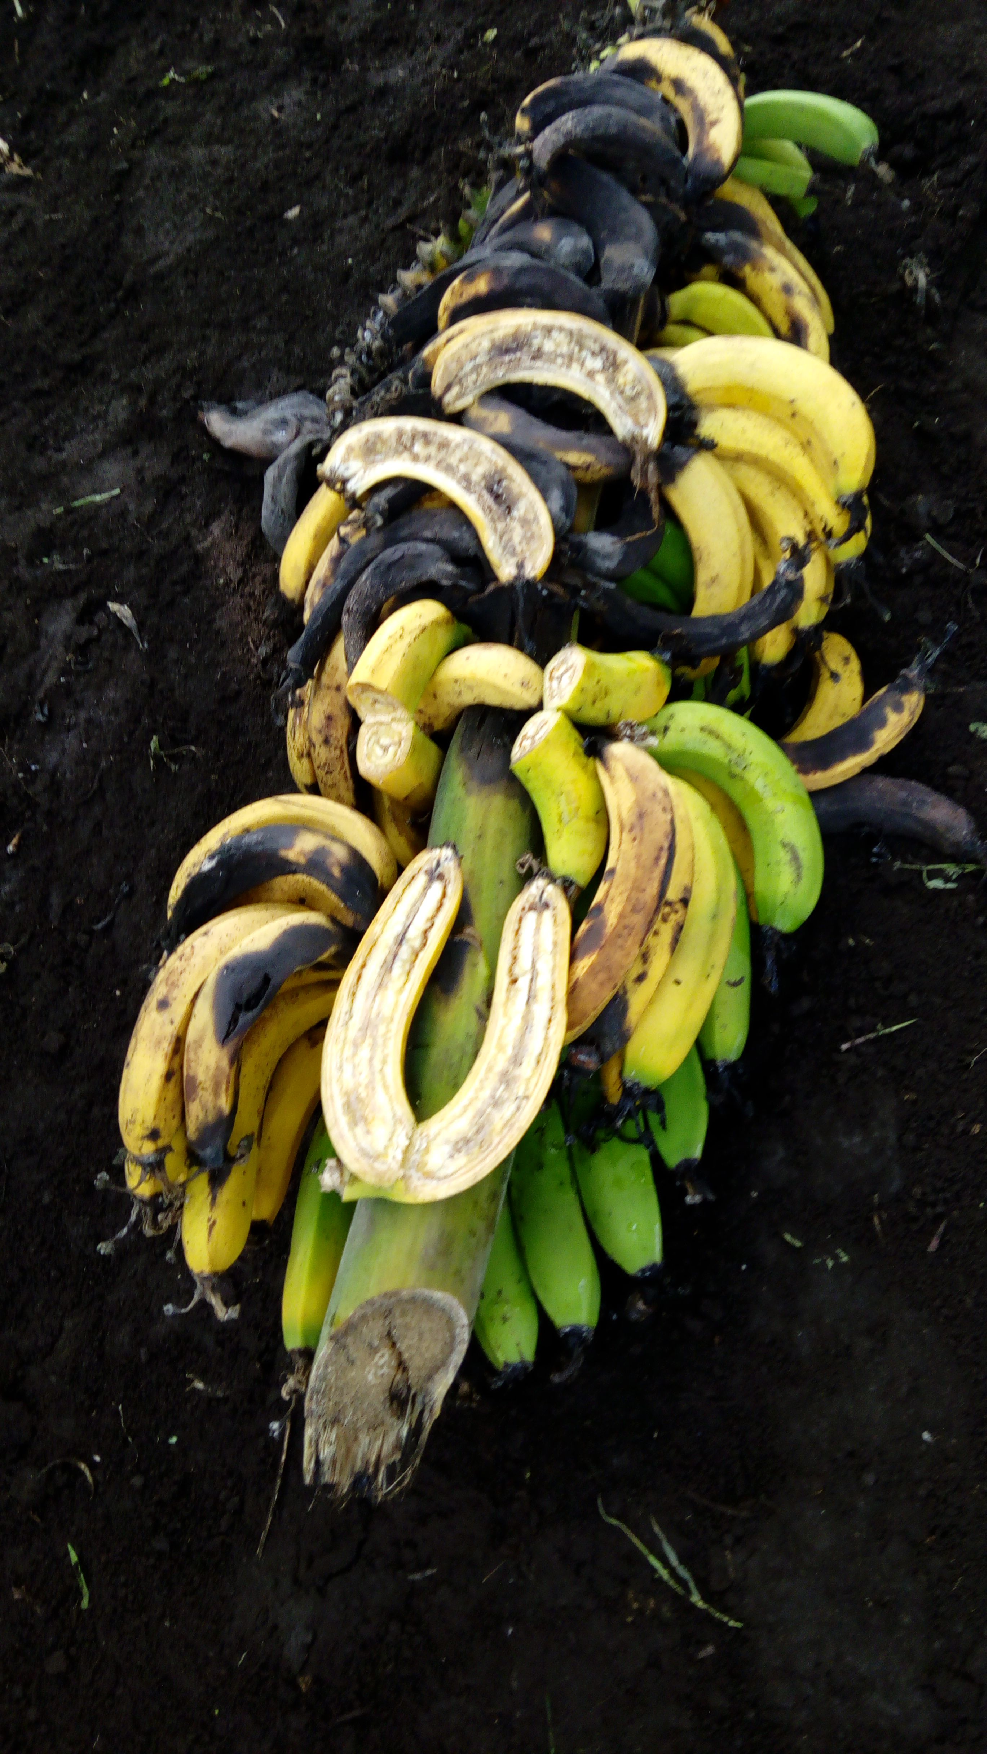
\includegraphics[width=0.9\linewidth, height=5cm]{Figures/bunch.pdf} 
\caption{BXW in banana fruit bunch}
\label{fig:subim1}
\end{subfigure}
\begin{subfigure}{0.5\textwidth}
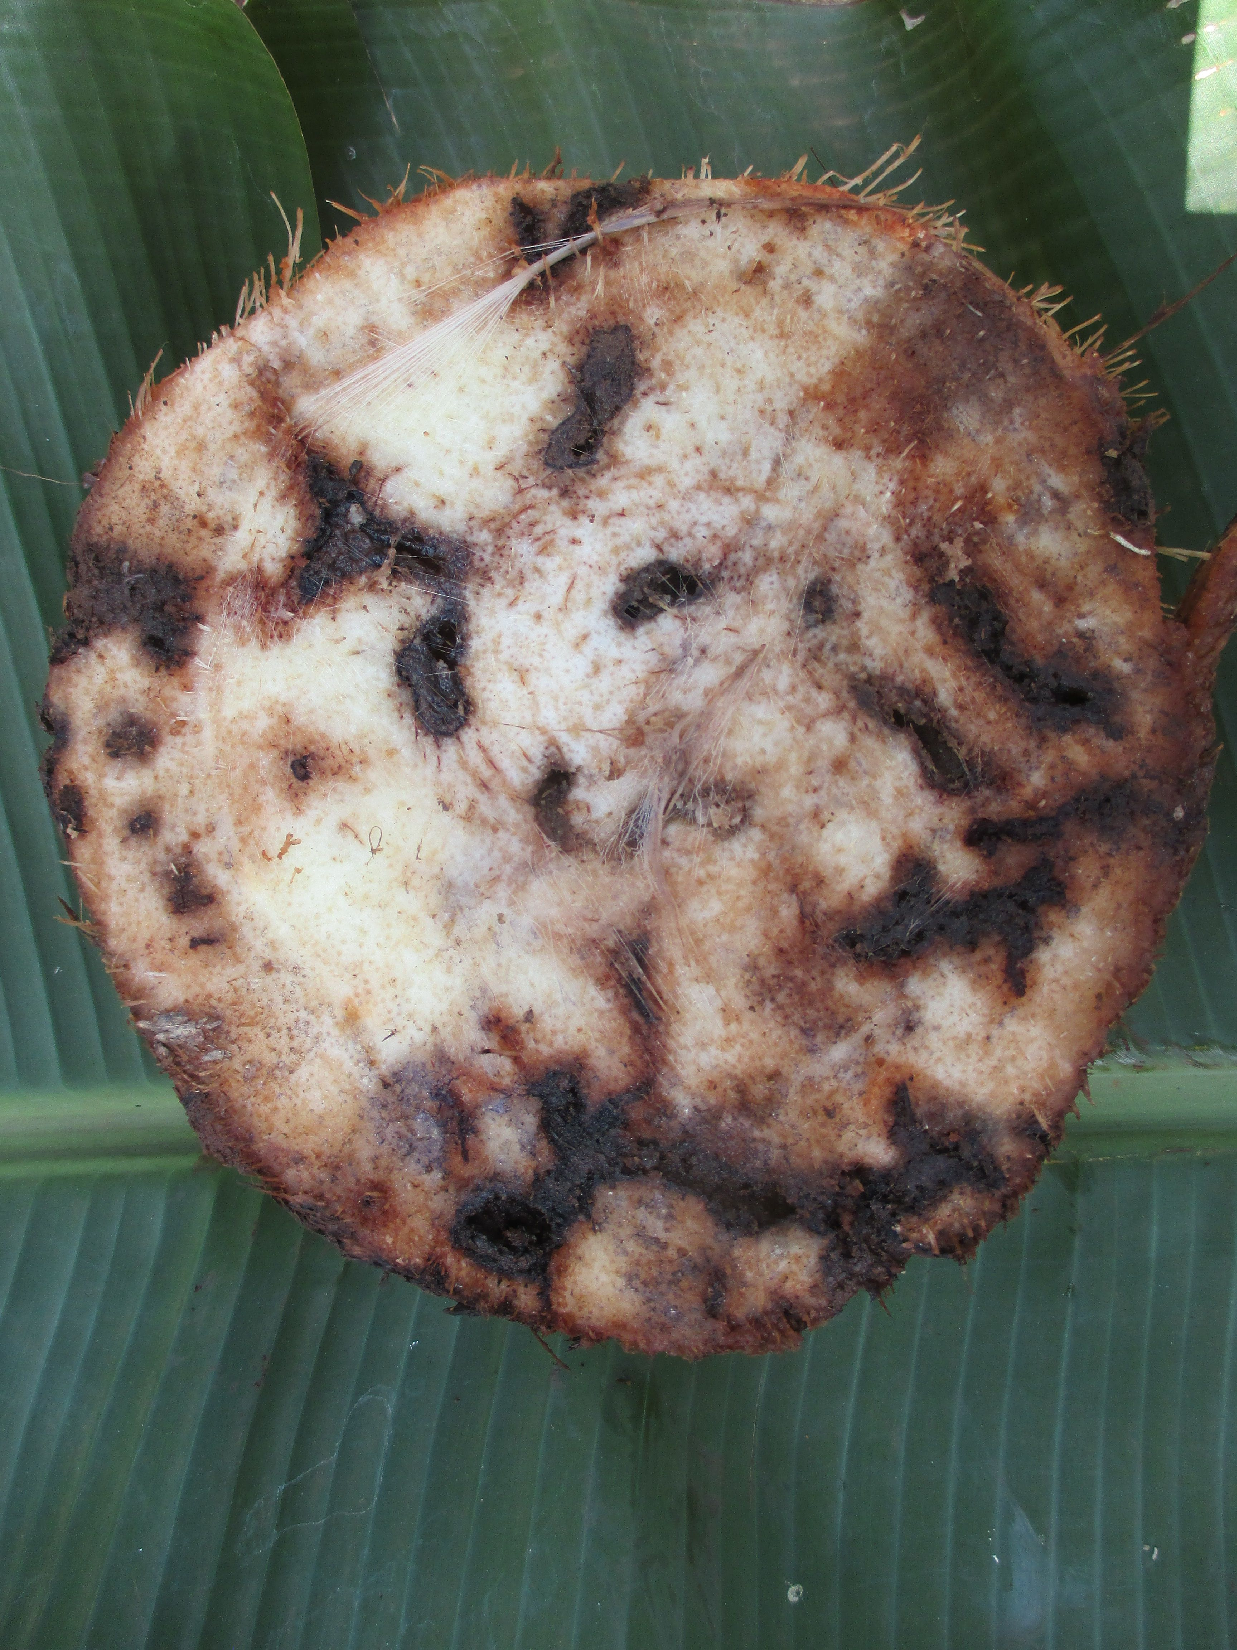
\includegraphics[width=0.9\linewidth, height=5cm]{Figures/corm.pdf}
\caption{Banana weevil effects in the corm}
\label{fig:subim2}
\end{subfigure}
 
\caption{Disease and pest impact in banana}
\label{fig:image2}
\end{figure}




Artificial intelligence (AI) with deep learning models \cite{goodfellow2016deep} are useful to help identify plant diseases by the plant’s appearance and visual symptoms\cite{camargo2009image}. Deep learning models can be embedded in smartphones to create applications that could alert farmers of the presence of a disease, lead to concerted control actions and thus potentially preventing a disease from spreading over large areas\cite{mohanty2016using}. Even though many of the developing country farmers around the world do not have access to these advanced tools, internet infiltration and smartphone penetration offer new outfits for in-field crop disease detection. The GMSA (Global System for Mobile Association) predicted that global smartphone subscriptions would reach 5 billion by 2020, of which nearly one billion in Africa (GSMA Intelligence, 2016). 
Mobile applications are promising to be excellent tools to support farmers in disease detection and crop management. The main problem with AI applications is that it is needed vast amounts of data to train the models and have reliable predictions, since in deep learning techniques specially in object detection models the main data source are images, it also need many images to learn the patterns. In real cases is very difficult to obtain a data set with enough and reliable images, because the images should be taken in different environmental conditions, different hours (morning, noon and afternoon) and by disease experts. 

As banana is one of the most important fruit crops around the world, it is needed to create easy tools to detect diseases using deep learning models, but there is a big problem and is the data acquisition as mentioned before, fortunately, traditional data augmentation methods have demonstrated  to be an excellent option to increase the number of images\cite{barbedo2018impact} but these approaches are just making the models more robust to orientation using the same original information, so creating new artificial information is the real call of duty, generated artificial data could improve not only the performance of the deep learning models but the generalization capabilities, and this is the scope for this work. To evaluate if artificial data is strong enough and a good option in order to increase the accuracy and the performance of deep learning models but also to ease the creation of new technology implemented in Banana for the future, following research questions have been generated: 
\begin{itemize} 
\item Traditional data augmentation techniques are enough to increase the performance of object detection deep learning models in banana disease detection?
\item Artificial data helps in disease diagnostic tasks?
\item How many images are needed to have a good performance in object detection deep learning models for banana diseases?
\item Combining real data with augmentation techniques and artificial data will improve the performance of object detection deep learning models?
\end{itemize}  